\documentclass{report}
\usepackage{graphicx}
\usepackage{fullpage}
\usepackage{titlesec}
\usepackage{amsmath}

\newcommand{\statenum}{533,482 }
\newcommand{\bbstatenum}{$BB($533,482) }
\newcommand{\bbstatenumcomma}{$BB($533,482, }
\newcommand{\bbstatenumperiod}{$BB($533,482. }

\setcounter{secnumdepth}{4}

\begin{document}

\title{A Relatively Small Turing Machine Whose Behavior Is Independent of Set Theory}
\author{Adam Yedidia}

\maketitle

\begin{abstract}

I present an explicit description of a Turing machine $G$ whose behavior cannot be proved in ZFC, assuming ZFC is consistent. In doing so, I give the first known upper bound on the highest provable Busy Beaver number in ZFC, assuming ZFC is consistent. In the process of creating $G$, I define a higher-level language, TMD, which is much more convenient for writing in than direct state manipulation, and explain in detail the process of compiling this language down to a Turing machine description. TMD is a well-documented language that is optimized for parsimony over efficiency. This makes TMD a uniquely useful tool for creating further Turing machines that verify mathematical statements. 

\end{abstract}

My thesis is split into two chapters. The first chapter explains \emph{what} was done: ZFC, Turing machines, G\"{o}del's incompleteness theorems, the Busy Beaver function, and general clarifications. The second chapter explains \emph{how} it was done: TMD, what intermediate steps are contained between the high-level language and the low-level Turing machine description, and the general algorithm for compilation.

\chapter{Concept}

\section{Background and Motivation \label{sec:background}}

\emph{Zermelo-Fraenkel set theory with the axiom of choice}, more commonly known as ZFC, is an axiomatic system invented in the twentieth which has since been used as the foundation of most of modern mathematics. It encodes arithmetic by describing natural numbers as increasing sets of sets. Because of its importance as the basic assumption from which most interesting mathematics is derived, it has been the object of plenty of study. \\

Like any axiomatic system capable of encoding arithmetic, ZFC is constrained by G\"{o}del's two incompleteness theorems. The first incompleteness theorem states that if ZFC is \emph{consistent} (it never proves both a statement and its opposite), then ZFC cannot also be \emph{complete} (it proves every true statement). To see that this is true, consider the statement $S$: ``This statement is not provable in ZFC.'' $S$ cannot be proved with ZFC, since if it was proven then it would be false! But if it cannot be proved with ZFC, then it must be true. Hence, there is a true statement in ZFC that cannot be proved in ZFC. \\

G\"{o}del's second incompleteness theorem states that if ZFC is \emph{sound} (it only proves statments that are true), then ZFC cannot prove its own consistency. To verify this, consider a scenario in which ZFC could prove its own consistency. Now suppose that the statement $S$ above was false. That would imply that $S$ \emph{is} provable in ZFC--which would mean ZFC can prove a falsehood, which is impossible! It follows that the statement $S$ above must be true. But if this conclusion follows from the assumption of ZFC's consistency, then it must be true that if ZFC can prove its own consistency, it can also prove $S$. However, it was established from the proof of the G\"{o}del's first incompleteness theorem that ZFC cannot prove $S$ and remain consistent! Thus, if ZFC is sound and can prove its own consistency, it must be able to prove $S$, so it must be inconsistent. But if ZFC is inconsistent and can prove its own consistency, it must not be sound! Therefore, assuming ZFC is sound, ZFC cannot prove its own consistency. J. Rosser was able to retain the proof while weakening the assumption of soundness to an assumption of consistency in 1936. \\ % TODO cite?

Because we as mathematicians have built modern mathematics on top of ZFC, we can reasonably be said to have assumed ZFC's soundness. This means that we must also assume that ZFC cannot prove its own consistency. This fact carries with it certain surprising conclusions. \\

In particular, consider a Turing machine $G$ that enumerates, one after the other, each of the provable statements in ZFC. Because ZFC is \emph{computable}, it follows that such a machine must exist. To describe how such a machine might be constructed, $G$ could iterate over each of the axioms of ZFC, applying each axiom in each possible way to the conclusion that had been reached so far. We might ask $G$ to halt if it ever reaches a contradiction; in other words, $G$ will halt if and only if it ever finds two provable statements in ZFC that contradict each other. Because we know that this machine will enumerate \emph{every} provable statement in ZFC, we know that it will halt if and only if ZFC is inconsistent. \\

It follows that $G$ is a Turing machine for which the question of its behavior (whether or not it halts when run indefinitely) is equivalent to the consistency of ZFC. Therefore, just as ZFC cannot prove its own consistency (assuming ZFC is sound), ZFC also cannot prove that $G$ will loop or halt. \\

This is intuitively very surprising. While the proof of the undecidability of the halting problem (see Section~\ref{sec:halting}) tells us that there cannot exist an algorithmic method for determining whether an \emph{arbitrary} Turing machine loops or halts, $G$ is an example of a \emph{specific} Turing machine whose behavior cannot be proven one way or the other using the foundation of modern mathematics. We as mathematicians and computer scientists think of ourselves as being able to determine how a given algorithm will behave if we are given enough to stare at it; despite this intuition, $G$ is a machine whose behavior we can never prove without assuming axioms more powerful than those generally assumed in most of modern mathematics. \\

This is only the first surprising fact that follows from G\"{o}del's second incompleteness theorem when applied to ZFC. In the next section, I discuss the Busy Beaver function and the implications on it from a machine like $G$.

\section{Turing Machines \label{sec:tm}}

Mathematians and computation theorists often make reference to a type of machine called a \emph{Turing machine}. Formally, a Turing machine is a 7-tuple of relevant values, one of which is the \emph{transition function}; informally, a Turing machine is a mathematical desciption of an algorithm. In 1936, Alonzo Church and Alan Turing independently proved what would eventually become known as the \emph{Church-Turing thesis}, which postulated that anything that could be done by a computer or by a human with pencil and paper, ignoring resource limitations, could also be done by Turing machine. Turing machines have since become a stand-in used by mathematicians for an algorithm, or a computer program. Because they provide a convenient common standard, because they make the notion of an algorithm rigorous, and because they are as powerful as any other computational machine, mathematicians have used Turing machines to reason about the limits of human computation for the last century. \\

There are many different competing definitions for Turing machines, each differing slightly from the other. For example, some definitions for Turing machines allow the machine to have a finite number of tapes; others only allow it to have one. Some definitions allow an arbitrarily large alphabet, while others only allow two symbols. Some definitions allow the tape head to remain in place, while others require it to move at every time-step. In most research regarding Turing machines, mathematicians don't concern themselves with which of these models to use, because any one of them can simulate the others, if a constant overhead in the number of states is allowable. Because the work of my thesis concerns at various points the exact number of states required to perform certain tasks, it is important to rigorously define what model of Turing machine is being used. \\

Formally, any $k$-state Turing machine used in this thesis is a 7-tuple $M = (Q, \Gamma, b, \Sigma, \delta, q_0, F)$, where: \\ \\
$Q$ is the set of $k$ \emph{states} $\{q_0, q_1, \dots, q_{k-2}, q_{k-1}, q_{\textrm{ACCEPT}}, q_{\textrm{REJECT}}\}$ \\
$\Gamma = \{0, 1\}$ is the set of \emph{tape alphabet symbols} \\
$b = 0$ is the \emph{blank symbol} \\
$\Sigma = \empty$ is the set of \emph{input symbols} \\\
$\delta = (Q \\ F) \times \Gamma \rightarrow Q \times \Gamma \times \{L, R\}$ is the \emph{transition function} \\
$q_0$ is the \emph{start state} \\
$F = \{q_{\textrm{ACCEPT}}, q_{\textrm{REJECT}}\}$ is the set of halting states. \\

In this thesis, a Turing machine's \emph{states} make up the Turing machine's easily-accessible, finite memory. The Turing machine's state is initialized to $q_0$. New states are entered according to the Turing machine's transition function. \\

The \emph{tape alphabet symbols} correspond to the the symbols that are can be written on the Turing machine's infinite tape. \\

The \emph{blank symbol} is the only symbol that can appear on the tape an infinite number of times. In my thesis, all Turing machines discussed are run on the \emph{empty input}, which means that all Turing machines discussed are run on a tape where every slot contains the blank symbol. \\

The \emph{input symbols} are the only symbols that can appear on the tape at initialization, other than the blank symbol. They encode the input to the Turing machine. Because all Turing machines discussed in my thesis are run on the empty input, no input symbols will appear on the tape at initialization. \\

The \emph{transition function} encodes the Turing machine's behavior. It is, in some sense, what encodes the algorithm itself. It takes two inputs: the current state of the Turing machine (an element of $(Q \\ F)$ and the symbol read off the tape (an element of $\Gamma$). It outputs three separate instructions: what state to enter (an element of $Q$), what symbol to write onto the tape (an element of $\Gamma$) and what direction to move the head in (an element of $\{L, R\}$). A transition function specifies the entire behavior of the Turing machine in all cases. \\

The \emph{start state} is the state that the Turing machine is in at initialization. \\

The \emph{set of halting states} is the set of states such that when the Turing machine enters one of these states, execution halts. The question of whether or not a Turing machine halts centers around whether or not a Turing machine will ever enter a state in this set when run indefinitely. Note that states in this set are not included as possible inputs to the transition function, but are included as possible outputs; this encodes the fact that while Turing machines can enter one of these states, they cannot leave them. 

\section{The Busy Beaver Function}

Consider the set of all Turing machines with $k$ states, for some positive integer $k$. In computability theory, we call a Turing machine $B$ a $k$-\emph{Busy Beaver} if when run on the empty tape as input, the following is true: \\ \\
-$B$ halts. \\
-$B$ has $k$ states. \\
-$B$ runs for at least as many steps before halting as all other halting $k$-state Turing machines. \\

In other words, a Busy Beaver is a Turing machine is a Turing machine that runs for at least as long as all other Turing machines with as many states as it. \\

The \emph{Busy Beaver function}, often written $BB(x)$, takes as input a positive integer $x$ and returns how many steps it takes for an $x$-Busy Beaver to halt. The Busy Beaver function has a lot of interesting mathematical and computational properties. To begin with, the Busy Beaver function is not a \emph{computable} function; in other words, there does not exist an algorithm that takes $x$ as input and returns $BB(x)$, for any value of $x$. This follows directly from the undecidability of the halting problem. Suppose an algorithm existed that could compute the Busy Beaver function; then, given a $k$-state Turing machine $M$ as input, we could compute $BB(k)$ and run $M$ for $BB(k)$ steps. If, after $BB(k)$ steps, $M$ had not yet halted, we could safely conclude that $M$ would never halt. Thus, if an algorithm $A$ existed to compute the Busy Beaver function, we could construct an algorithm $A'$ to tell us if an arbitrary Turing machine will halt. Because $A'$ cannot exist (see Section~\ref{sec:halting}), $A$ cannot exist either. \\

By the same proof as the one above, we also know that $BB(x)$ must grow faster than any computable function. (To check this, assume that some computable function $f(x)$ grows faster than $BB(x)$, and substitute $f(k)$ for $BB(k)$ in the rest of the proof.) This is a very impressive feature for a function to have, because there exist computable functions, such as the well-known Ackermann function, that are known to grow extremely quickly. \\

For most purposes, when reasoning about Turing machines, it is unnecessary to define precisely what model of Turing machine is being used. Single-tape Turing machines can simulate multi-tape Turing machines, and vice-versa; Turing machines using a two-symbol alphabet can simulate Turing machines using an arbitrarily large but finite alphabet; Turing machines whose heads cannot remain in place after a single time-step can simulate Turing machines whose heads can, and vice-versa. In each of these cases, however, the simulation may require some overhead in the number of states. When discussing explicit values of the Busy Beaver function, the exact number of states used in the Turing machine is relevant. For this reason, any discussion of the Busy Beaver function must include a corresponding Turing machine model. \\

The most common Turing machine model associated with the Busy Beaver function is also the weakest Turing machine model generally discussed by mathematicians; that is, it concerns a single-tape, two-symbol Turing machine that cannot remain in place. This model is formally defined in Section~\ref{sec:tm}. % TODO cite this?
In the remainder of this section, explicit values of the Busy Beaver function will be discussed. For all of these explicit values, we assume that this Turing machine model is the one being used. \\

Partly because the Busy Beaver function grows so quickly, and partly because the finding the value of Busy Beaver of $x$ for a given $x$ requires so much work (one must fully explore the behavior of all $x$-state Turing machines), few explicit values of the Busy Beaver function are currently known. The known values are as follows: \\

$$BB(1) = 1$$
$$BB(2) = 6$$
$$BB(3) = 21$$
$$BB(4) = 107$$

Beyond these four, no values of the Busy Beaver function have been proven. However, lower bounds exist for $BB(5)$ and $BB(6)$. Researchers are currently working on pinning down the value of $BB(5)$ exactly, and consider it to possibly be within reach:

$$BB(5) \ge 47,176,870$$
$$BB(6) \ge 7.4 \times 10^{36534}$$

The current state of human knowledge is that the first four Busy Beaver values are known. Another way to say this is that modern mathematics has established a \emph{lower bound} of 4 on the highest provable Busy Beaver value. In my thesis, I prove the first known \emph{upper bound} on the highest provable Busy Beaver value in ZFC; that is, I give a value of $x$ such that the value of $BB(x)$ cannot be proven in ZFC. \\

The existence of such an upper bound is very intuitively surprising; one might expect that while no algorithm may exist to compute $BB(x)$ for \emph{any} value of $x$, we could find the value of $BB(x)$ for any \emph{specific} value of $x$ using a procedure similar to the one we used to find the value of $BB(x)$ for $x \le 4$. The reason that such an upper bound must exist is closely tied to the existence of a machine like the G\"{o}delian machine $G$, as described in Section~\ref{sec:background}. Suppose that $G$ has $k$ states. Because $G$'s behavior (whether it halts or loops) cannot be proven in ZFC, it follows that the value of $BB(k)$ also cannot be proven in ZFC; if it could, then a proof would exist of $G$'s behavior in ZFC. Such a proof would consist of a \emph{computation history} for $G$, which is an explicit step-by-step description of $G$'s behavior for a certain number of steps. If $G$ halts, a computation history leading up to $G$'s halting would be the entire proof; if $G$ loops, then a computation history that takes $BB(k)$ steps, combined with a proof of the value of $BB(k)$, would constitute a proof that $G$ will run forever. \\

For my thesis, I constructed a machine like $G$, for which a proof that $G$ runs forever would imply that ZFC was consistent. In doing so, I found an explicit upper bound on the highest Busy Beaver value provable in ZFC. My machine, which I shall refer to as $G$ hereafter in the paper, contains \statenum states. Therefore, we will never be able to prove the value of \bbstatenum without assuming more powerful axioms than the ones assumed in most modern mathematical proofs.

\section{A Description of $G$}

In Section~\ref{sec:background}, I described a G\"{o}delian Turing machine that would be \emph{independent of ZFC}; it would not be possible to prove that this machine would halt or wouldn't halt using the axioms of ZFC, assuming that ZFC was consistent. I suggested that one might build this machine by instructing the machine to start with an identity and apply the axioms of ZFC repeatedly in each possible way so as to enumerate every statement ZFC could ever prove, and to halt if ever a contradiction was found. While the idea for this method is simple, to actually construct such a machine would be very involved, because it would require creating a language in which to encode the axioms of ZFC that could be stored on a Turing machine tape. \\

Thankfully, a simpler method exists for creating $G$. Prof. Harvey Friedman was able to derive a graph-theoretical statement whose truth cannot be proved in ZFC if ZFC is consistent[1], and which is false if ZFC is not consistent. (Note that these two properties are also true of the statement, ``ZFC does not contain a contradiction.'' These two properties are what we ultimately need to prove an upper bound on the highest provable Busy Beaver value in ZFC!) The statement is as follows: \\

\emph{For all $k, n, r \ge 0$, every order invariant graph on $[Q]^{\le k}$ has a free $\{x_1,\dots,x_r,ush(x_1),...,ush(x_r)\}$ of complexity $\le 8knr!$, each
$\{x_1, \dots, x_{(8kni)!}\}$ reducing $[x_1 \cup \dots \cup x_i \cup \{0,\dots,n\}]^{\le k}$.}

In this statement, an \emph{order invariant graph} is a graph containing an infinite number of nodes. In particular, it has one node for each finite set of real numbers of size $k$ or smaller. In every description of nodes that follows, the term \emph{node} refers both to the object in the order invariant graph and to the set of numbers that it represents. \\

Additionally, in an order invariant graph, two nodes $(a,b)$ may have an edge between them if and only if each other pair of nodes $(c,d)$ that is \emph{order equivalent} with $(a,b)$ have an edge between them. Two pairs of nodes $(a, b)$ and $(c, d)$ are \emph{order equivalent} if $a$ and $c$ are the same size and $b$ and $d$ are the same size and if for all $1 \le i \le |a|$ and $1 \le j \le |b|$, the $i$-th element of $a$ is less than the $j$-th element of $b$ if and only if the $i$-th element of $c$ is less than the $j$-th element of $d$. \\

To give a few trivial examples of order invariant graphs: the empty graph is an order invariant graph, as is the complete graph. A graph being order invariant imposes the restriction that \emph{under certain circumstances, if $a$ and $b$ have an edge between them, $c$ and $d$ must too}--a condition which, no matter the circumstances asked, is satisfied by both the complete and the empty graph. Non-trivial examples of order invariant graphs are more difficult to fully describe, because of the fact that they contain an infinite number of nodes; however, subgraphs of non-trivial order invariant graphs can be helpfully described. \\ 

% TODO describe a subgraph of a non-trivial order invariant graph

The \emph{ush()} function takes as input a set and returns a copy of that set with all non-negative numbers in that set incremented by 1. \\ 

A number of \emph{complexity} at most $c$ refers to a number that can be written as a fraction $a/b$, where $a$ and $b$ are both integers less than or equal to $c$. A set has complexity at most $c$ if all the numbers it contains have complexity at most $c$. \\ 

Finally, to quote [1]: \\

\emph{A set of vertices $X$ reduces a set of vertices $Y$ if and only if for all $y \in Y$, either $y \in X$ or there is an $x \in X$ such that ($x E y$ and $\max(x) \le \max(y)$)}. \\

In order to show that \bbstatenum was not provable in ZFC assuming that ZFC is consistent, I constructed a Turing machine, that I will hereafter call $G$, that loops if the statement above is true, and halts if it is false. Because $G$ contains \statenum states, a proof of \bbstatenum would imply a proof of the statement's truth in ZFC (the proof would consist computation history that shows $G$ running for \bbstatenum steps, and a proof of the value of \bbstatenum).

\section{Parsimony}

To construct $G$, a program that checks the correctness of Statement~\ref{eq:friedman} appears at first to be a daunting task. In particular, it is impossible for the program to check the correctness of the statement for large $k$, $n$, and $r$ efficiently; note that the statement requires us to check all subgraphs of complexity $(8knr)!$. This requires us to enumerate all fractions with numerators and denominators of size at most $(8knr)!$, for a total of $\Theta((8knr!)^2)$ different fractions! Plainly, this is not a remotely tractable task. \\

Fortunately, for the purpose of the proof that this paper hopes to create, tractability is not a concern! It is unimportant that $G$ be efficient; if the goal was in fact to find a contradiction in ZFC, there would be much better ways to do it than to enumerate every provable statement in ZFC, or to verify the truth of arcane graph-theoretical statements. Moreover, even if the best way to find a contradiction in ZFC was by mechanically running a computer program, it would be far better to implement the the computer program in software directly, rather than implementing it as a Turing machine and simulating the Turing machine in software for as many steps as possible. \\

Crucially, the goal of my thesis is \emph{not} to find a contradiction in ZFC. Instead, it is to construct a proof of the unprovability of large enough Busy Beaver values in ZFC, through the construction of a Turing machine that cannot be proved to loop in ZFC if ZFC is consistent. It is entirely unimportant to this task that the Turing machine how quickly this machine loops. \\

It is, however, important that this program's description be \emph{parsimonious}--that is, that the program use as few states as possible. The fewer states in $G$, the stronger the upper bound on the highest provable Busy Beaver value. \\

In most theoretical algorithmic study, efficiency is the primary concern. On occasion, space usage is also an important concern. In the pursuit of a description for $G$, however, parsimony is instead the only thing that matters. This leads to a lot of unorthodox design decisions, which are gone into in detail in Chapter~\ref{sec:implementation}. I will note, however, that the point of view of optimizing for \emph{simplicity} is a completely different mindset. The closest thing I can think of that I have seen done previously is the practice of ``code-golfing'': a recreational pursuit adopted by some programmers in which the goal is to produce a piece of code written in a given programming languages, using as few characters as possible. The goal of designing a Turing machine with as few states as possible to accomplish a certain task, without concern for the machine's efficiency or space usage, can be thought of analogous to code-golfing with a particularly low-level programming language.

\section{Frequently Asked Questions \label{sec:faq}}

The study of axiomatic systems such as ZFC can often be confusing. This section is meant to help possible misunderstandings that the reader may have about this paper's result. \\

\textbf{Q: I claim that the value \bbstatenum can't be proven in ZFC because if it could, then a proof would exist of Statement~\ref{eq:friedman}'s truth in ZFC. But what if the statement was false? Wouldn't a proof of the statement's falsehood exist in ZFC, with or without knowing the value of \bbstatenumcomma by simply give the computation history of $G$ until $G$ halts?} \\

A: If the Statement~\ref{eq:friedman} was false, there would indeed exist a proof of the statement's falsehood. However, remember that this statement, just like the similar statement ``ZFC does not contain a contradiction,'' has the property that ZFC must be inconsistent if it is false! Therefore, as long as ZFC is consistent, it cannot contain a proof of Statement~\ref{eq:friedman}'s truth \emph{or} falsehood. It cannot contain a proof of Statement~\ref{eq:friedman}'s truth, because then it would contain a proof of its own consistency, which no consistent axiomatic theory can have. And it cannot contain contain a proof of Statement~\ref{eq:friedman}'s falsehood, because that would prove that ZFC is inconsistent! \\

\textbf{Q: Does my result mean people will never know the value of \bbstatenum with certainty?} \\

A: Well, it depends on what one means by ``knowledge''! If we restrict ourselves to the axioms of ZFC, we can never \emph{prove} the value of \bbstatenumperiod But if we are willing to assume more powerful axioms than ZFC, then we certainly could! For example, if we are willing to assume an axiom that states ZFC's consistency (which may be reasonable, since most mathematicians believe that ZFC is consistent), then it's entirely possible that we could prove the value of \bbstatenum from within the axiomatic system of (ZFC + $Con($ZFC)). And although most mathematical proofs use only ZFC as axioms, historically, when people have assumed more powerful axioms, it hasn't caused mathemticians to truly doubt the result that was produced. For example, in Wiles' proof of Fermat's Last Theorem, more powerful axioms than ZFC were used, and it wasn't a serious issue. %TODO cite \\

\textbf{Q: So if we can just assume axioms more powerful than ZFC to prove the value of \bbstatenumcomma what's the significance of saying that \bbstatenum can't be proved in ZFC?} \\

A: Although it is possible to simply assume new and more powerful axioms to prove desired results, it's not a very convincing way to ``prove'' things! And crucially, there's no algorithmic way of ``safely'' assuming new mathematical axioms. Each new mathematical axiom assumed carries with it a genuine risk of introducing an inconsistency, such as Russell's paradox, which ZFC cleverly sidesteps. % TODO cite
There's no larger mathematical consensus of where exactly our knowledge ends; rather, there is a continuous spectrum of increasingly powerful axiomatic theories, each of which is riskier than than the previous one. ZFC happens to be a particularly salient point on that spectrum, because it is well-known, contains enough power to prove most of modern mathematics, and is generally considered very likely to be consistent. I decided to write my proof for ZFC in particular, but no matter where I had decided to draw that line, there would always have been some value $x$ for which $BB(x)$ would be unprovable. 

\chapter{Implementation \label{sec:implementation}}

\section{Overview}

This chapter is devoted to explaining how to write parsimonious Turing machine descriptions. At the start of this chapter, I provide an overview of the compilation process, an explanation of major design decisions, and ideas for further directions to pursue. Following that, I provide a detailed description of the TMD language and the compilation algorithm. \\

A two-symbol, single-tape Turing machine is very unwieldy. It is very inconvenient to program it directly, manipulating each state by hand. Instead, I created a simple higher-level language, which I named Turing Machine Descriptor (TMD). In addition, I wrote two pieces of code: a compiler written in Python that transforms TMD into a description of a 2-symbol, single-tape Turing machine, and a program written in TMD that encodes Statement~\ref{eq:friedman}. \\
 
The compiler used and referenced in this paper has as its goal to convert a program written in TMD into a description of Turing machine running on a single tape and using a 2-symbol alphabet. In between, the code is passed through two intermediate stages: a description of a Turing machine running on multiple tapes using a 3-symbol alphabet, and a description of a Turing machine running on a single tape using a 4-symbol alphabet. A detailed diagram illustrating this process is visible in Figure~\ref{fig:process}. \\

In this chapter, each of the four representations will be described in turn, from highest- to lowest-level. Additionally, detailed explanations will be given for how the conversion of one representation to the one immediately below it is done.

\begin{figure} 
\begin{center} 
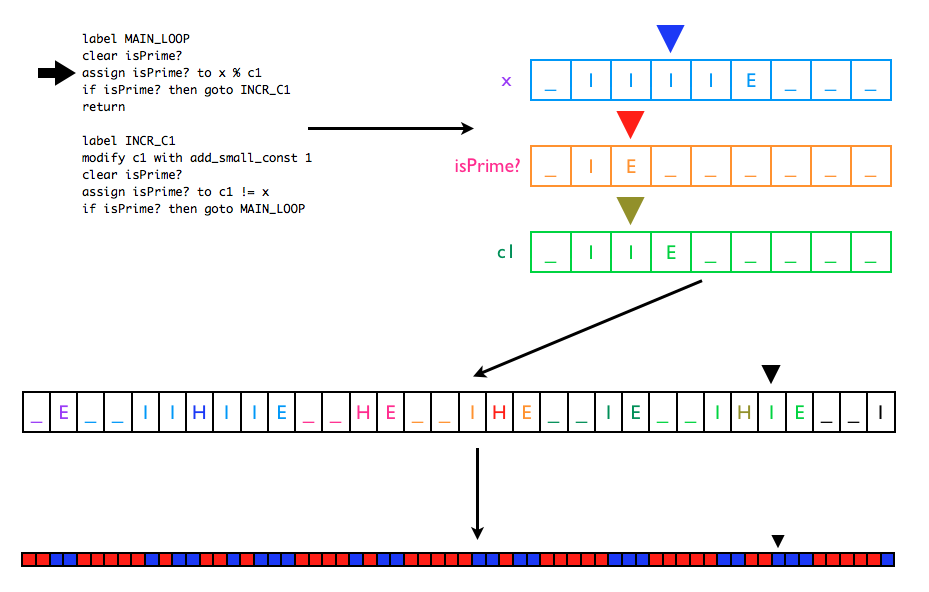
\includegraphics[height=3.25in,width=5in,angle=0]{figs/process.png} 
\caption{This diagram illustrates each of the steps in the conversion between a program written in TMD and a description of a single-tape Turing machine with a binary tape alphabet.\label{fig:process}} 
\end{center} 
\end{figure}  

\section{Major Design Decisions}

The goal of my thesis is ultimately to produce a \emph{parsimonious} Turing machine: a Turing machine with minimal number of states. The design of the compiler is informed by this fact. \\

\subsection{The Tape-Variable Relationship}

The first major design decision was to use a higher-level abstraction of a multi-tape Turing machine to represent the variables in a convenient manner. Later, the multi-tape Turing machine is automatically converted to a single-tape Turing machine.  \\

In the multi-tape Turing machine, each variable is given its own tape. This makes it very easy to keep the values of each variable separate. Allowing separate variables in the compiled language is crucial for allowing standard programming techniques to be used. \\

There are several different possible definitions of the behavior of a multi-tape Turing machine that are possible to use. Perhaps the most common representation of a multi-tape Turing machine is the one in which each of the heads on each of the different tapes reads a symbol simultaneously, and each head is allowed to move right or left based on the combination of symbols that was read. Although this representation is very powerful, it is very expensive in terms of the number of states used--the number of lower-level states required is exponential in the number of tapes $t$ in the Turing machine, which in this case is equal to the number of variables used in the program the programmer wants to write. This is because each of the different $|\Sigma|^t$ different possible combinations of symbols needs to be considered ($\Sigma$ is the tape alphabet). \\

Instead of this powerful but unwieldy representation, I chose a representation that is slightly weaker but much more parsimonious. Each of the states $s$ in the higher-level multi-tape Turing machine has associated with it a single tape $T_s$. State transitions out of $s$ can only depend on the symbol read from $T_s$, and not on the symbols on the other tapes in the other Turing machines. In addition, after the symbol is read from $T_s$, only the tape head on $T_s$ can move left or right; other tapes' tape heads must remain in place. However, state transitions out of $s$ may transition to states that are associated with other tapes. This is how the behavior of the Turing machine can make use of multiple tapes at once: it can read them each in sequence and make a decision based on what was read from each tape. \\

\subsection{Unary}

The second major design decision that was made was to encode all integers in \emph{unary}: base-one notation. In other words, 1 is represented by ``\texttt{1},'' 2 is represented by ``\texttt{11},'' 3 by ``\texttt{111}'' Unlike representations of numbers in bases greater than one, which take space logarithmic in the value of the number being represented, numbers represented in unary take space linear in the value of the number being represented. As a result, the Turing machine produced by my compiler is exponentially slower and less space-efficient than it might have been with a more efficient numerical representation. However, it is also substantially more parsimonious. Algorithms for computing arithmetic operations in unary are substantially simpler than their binary counterparts, and in this situation, simplicity is all that counts. \\

As an example, consider the problem of integer divison. In binary, a series of complicated subtractions must be done to compute \texttt{a / b} in polynomial time. On a multi-tape Turing machine with the numbers written in unary, however, the problem becomes far simpler. If \texttt{a} is written on tape $T_a$ and \texttt{b} is written on tape $T_b$, and the output is expected to go on tape $T_c$, all that is necessary is to advance the heads on both $T_a$ and $T_b$ repeatedly. If the head on $T_b$ reaches the end of \texttt{b}'s representation, increment \texttt{c} and return the head on $T_b$ to the beginning of \texttt{b}. If the head on $T_a$ reaches the end of \texttt{a}'s representation, the algorithm terminates. \\

Although unary representation is very inefficient, it is the best way to write numbers that are subject to arithmetic operations and other manipulations if the goal is to make the algorithms for those manipulations as simple as possble. Happily, simplicity helps both from the point of view of minimizing states in the ultimate Turing machine, and from the point of view of making the programming of the compiler easy. \\

\subsection{Functions \label{sec:functions}}

The third major design decision that was made was to allow non-recursive functions. Originally, the plan was to have no functions at all, because I didn't think that I would need to reuse functions very often, and assuming the functions aren't being reused, allowing functions does not help save the amount of code written. Over the course of writing the program, however, it quickly became clear that functions play a crucial role in compartmentalizing a large program into easily-testable sections. \\ 

In the current version of the compiler, functions are compiled in a way that is equivalent to \emph{inlining} every function and then compiling the resulting program. (To \emph{inline} a function means to splice the code of the function into the place that the function was called.) This means that a separate set of states needs to be made for every call of each function, because the function's return address has been ``hard-coded'' into the set of states, instead of stored on the tape. Note that using this design choice, recursive functions (functions that directly or indirectly call themselves) are impossible: to inline such a function would cause an infinite loop. \\

Another possible choice for function processing would be to write the function stack directly onto the tape. In other words, instead of creating a set of states for every function call, simply create a set of states for every function proper, and write the current line number and current function on the tape. Whenever a function call occurs, push a representation of the return address onto the stack on the tape. When a function returns, return to the return address written at the top of the stack and remove it. \\

Because this approach creates a set of states for every line of code written across any function, instead of a set of states for every line of code multiplied by the number of times the surrounding function is called, writing the stack onto the tape can potentially be exponentially more parsimonious. In particular, in the case when the program contains $k$ programs $f_1, f_2, \dots, f_k$, and for each $1 \le i < k$, $f_i$ calls $f_{i+1}$ twice, the states associated with $f_k$ will appear $2^k$ times in the compiled Turing machine using the inlining method, but will only appear once using the stack-on-tape method. In addition, the stack-on-tape allows for the use of recursive functions.\\

In general, in the graph where each function in the program is given its own node, and where a directed edge is drawn from function $f_i$ to function $f_j$ for each time that $f_i$ calls $f_j$, the number of times that the code of $f_j$ will appear in the ultimate compiled program using the inlining method will be proportional to the number of paths from the main function to $f_j$ in the graph. Note that a recursive function corresponds to a cycle in the graph, and therefore to an infinite number of different paths! Note, also, that even if the graph is acyclic, the number of paths to $f_j$ can potentially be exponential in the size of the graph. \\

What, then, is the advantage of the inlining method? Besides being easier to implement from the point of view of designing the compiler, the only advantage is that it avoids the overhead of writing the function stack and line number on the tape, and needing to read it each time a line of code is executed. Additionally, if each function is only ever called once, inlining is no worse than writing the stack on the tape. Because most of the functions in my program were only going to be used once and were separated from each other mainly for the purpose of making testing easier, inlining was a natural choice for this thesis. For a different application in which functions were going to be reused a lot, or in which recursive functions were very important or much simpler than using loops, writing the stack on the tape might have been a much better choice than inlining. \\

Note that if a potential program repeats functions calls rarely, but occasionally, it is possible to use inlining and avoid copying the entire body of the function twice in the compiled program via a programming technique called \emph{loading}. In order to use this technique, a programmer can merge the two function calls into a single function call, with an instruction to call the function twice; after the first call to the function, the programmer can give the instruction to \emph{load} the second function call's arguments into the inputs to the function. I used this technique a handful of times in the design of $G$ to save states on what would have been a duplicate function call. If the programmer is finding herself doing this repeatedly, however, it is better to use the stack-on-tape method. One can think of loading as using the stack-on-tape method locally, with a single bit on the tape encoding the ``return address'' of the function. % TODO maybe give an example of loading?

For a side-by-side comparison of how a compiled program would look using the inlining and the stack-on-tape methods, see Figs.~\ref{fig:code} and~\ref{fig:compiled}.

\begin{figure} 
\begin{center} 
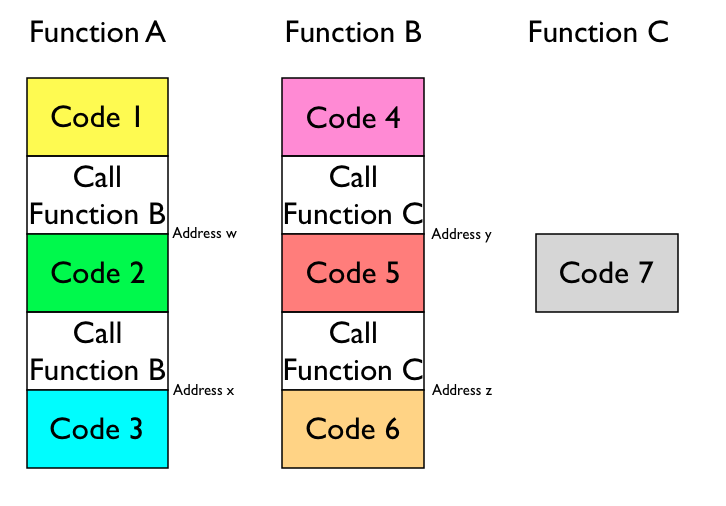
\includegraphics[scale=0.6]{figs/code.png} 
\caption{This is a visual representation of a program that spans three functions. The main function, Function A, calls Function B twice, and Function B calls Function C twice. Commands that are not function calls are labeled ``Code 1'' through ``Code 7.'' \label{fig:code}} 
\end{center} 
\end{figure}

\begin{figure} 
\begin{center} 
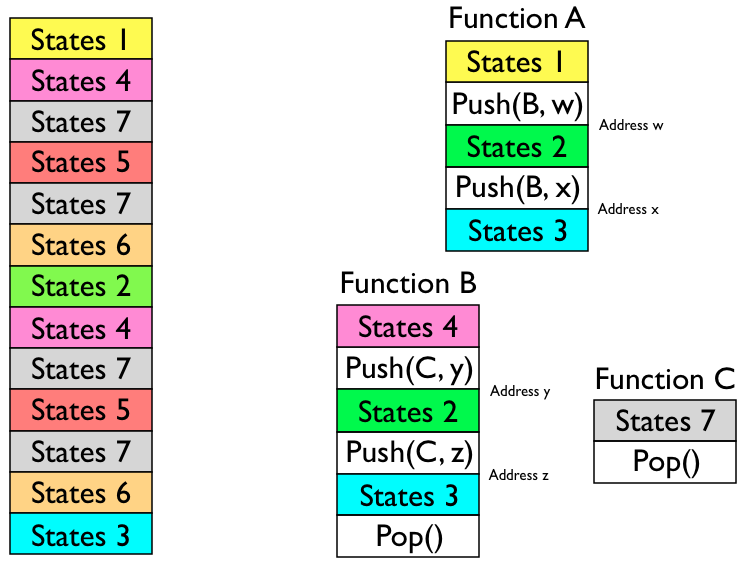
\includegraphics[scale=0.6]{figs/compiled.png} 
\caption{This is a visual representation of the compiled output of the program from Figure~\ref{fig:code}. On the left is the output of the compiler assuming the inlining method is used, while on the right is the output of the compiler assuming the stack-on-tape method is used. Note that the program flow of the compiled machine on the left is easier to understand; the program flow of the compiled machine on the right depends on what function is at the top of the stack. However, note also that if the set of states that represents ``Code 7,'' ``States 7,'' is very large, the stack-on-tape method is much more parsimonious than the inlining method in this case. On the left, ``States 7'' appears four times, but on the right it only appears once. \label{fig:compiled}} 
\end{center} 
\end{figure}

\section{Future Directions}

There are still countless improvements that can be made to the work in this thesis. The improvements can be separated into three different possible directions:  \\ \\
-Improving the TMD language to be more powerful and flexible \\
-Simplifying the final Turing machine, thereby tightening the upper bound of \statenum on the maximum computable Busy Beaver value \\
-Finding more upper bounds based on other axiomatic systems \\

\subsection{Improving TMD}

TMD is a relatively weak language with a lot of awkward aspects. For example, TMD does not support complex arithmetical expressions, either in assignment or as part of an \texttt{if} statement. Ideally, arbitrary expressions could be used in any of these places, to make TMD programs much shorter and less wordy. \\

Additionally, the fact that variables need to have a value of 0 before they can be reassigned is an annoyance. This aspect of TMD exists because sometimes the programmer already knows that the variable has a 0 value, so it would be wasteful to ``build in'' setting the value of the variable to 0 before reassignment. However, it would be far more convenient if the compiler could automatically recognize most of the situations where the variable is guaranteed to have a 0 value (such as when it hasn't been touched since declaration) and automatically forgo clearing the variable's value in those situations. \\

Finally, it would be very nice if \texttt{while} and \texttt{for} loops were possible in TMD, to make programs cleaner and easier to read. While \texttt{goto} statements are very natural from the point of view of simplicity of compilation, they tend to lead to to bad programming habits and inscrutable code. Providing programmers with the option of using \texttt{while} loops instead would make the job of debugging TMD programs easier. 

\subsection{Simplifying $G$}

The final Turing machine, $G$, whose behavior cannot be proven in ZFC, is not as parsimonious as it could be. At a basic level, the process of building a general-purpose compiler to Turing machines and then using that general-purpose compiler to create a specific program cannot possibly be as parsimonious as building the specific program directly. Abandoning the rigid abstraction barrier between the multi-tape and the single-tape abstraction, for example, is certain to make the resulting program more parsimonious, because it makes the programmer strictly more powerful than she was before. \\

However, this improvement in the number of states in the Turing machine comes at a tremendous cost in programmer effort. Abstraction barriers and modularity may not be ``optimal'' in the cosmic sense of the term, but they are often a necessary for completing the program without errors in a reasonable time-frame. \\

Nonetheless, there are always more optimizations that are possible from the point of view of improving the number of states. To start with, writing the function stack on the tape and trying as much as possible to rewrite different functions to reuse the same code is likely to result in a major savings in terms of the number of states. Although I rarely call identical functions in the final program, there are many instances where I call two very similar functions at different points in the program. When those functions are complex enough, it becomes worth it to build a single function capable of running both depending on its inputs, and calling that function twice with different arguments each time. Assuming the stack-on-tape method of compiling functions is being used (see~\ref{sec:functions} for a description of this method), this will most likely result in the number of states in the final program being substantially reduced. \\

Additionally, making the compiler more parsimonious at each stage is a good way to improve the upper bound presented in this thesis. In particular, the transformation from a 4-symbol Turing machine to a 2-symbol Turing machine has possible improvements that would likely result in a reduction of state usage by a factor of 1.5 or more; see Section~\ref{sec:mstots} for the details on what can be improved in the behavior of that compiler. \\

Naturally, there are most likely many other improvements that can be made to both the program and the compiler that would reduce the state usage of the result that I simply haven't yet thought of. Turing machines are so different in character from traditional programming languages that even the ways I think about variables and computation are ill-suited to the medium.

\subsection{Exploring Other Axiomatic Systems}

As was explained in Section~\ref{sec:faq}, the choice of ZFC as the axiomatic system to use was somewhat arbitrary. There are many different possible axiomatic systems that could have been used as ``the foundation of modern mathematics''; for most purposes, Peano Arithmetic (PA), a weaker axiomatic system than ZFC, is enough to prove interesting mathematical statements. Prof. Harvey Friedman has even conjectured that the still weaker system of Elementary Function Arithmetic (EFA) could be used to prove every theorem published in the \emph{Annals of Mathematics}. This includes Fermat's Last Theorem, whose only known proofs currently assume \emph{Grothendieck universes}, which require stronger axioms even than ZFC.  \\

It could therefore be interesting to find the upper bounds on the highest Busy Beaver values provable using these other systems of axioms--PA, EFA, and ZFC with Grothendieck universes. One presumes that the upper bounds will be tighter for the weaker systems of axioms and looser for the stronger systems of axioms; this could give us a sense of how much ``power'' is gained with each new assumed axiom. We could even find the strongest assumptions made by any theorem published in the \emph{Annals of Mathematics}, and find an upper bound on the highest Busy Beaver value provable using only those assumptions, to establish the full range of weak to strong.\\

This kind of further research would be helpful to give researchers a numerical value to assign to the strength and weakness of the assumptions of these various axiomatic systems--and possibly use that value to gain a sense of the resulting risk of an inconsistency being present. Prof. Harvey Friedman has helpfully created many different relatively-easy-to-program statements who, like Statement~\ref{eq:friedman}, cannot be proved in each of various different axiomatic systems. With Prof. Friedman's statements and my compiler, the work required to prove these new upper bounds is smaller than it ever has been.

\section{TMD}

The top-level representation is a program written in the TMD language, which is a language created and designed explicitly for use in this project. TMD is altogether not unlike Assembly Language, although it is more powerful in some ways and weaker in others. \\

TMD code can be processed in two different ways. First, it can be \emph{interpreted}; that is, it can be directly evaluated line-by-line. This is generally done to verify a program's correct behavior, and to correct errors which would result in thrown exceptions in the interpreter but might lead to undefined behavior in the compiled Turing machine (because the compiled Turing machine is optimized for parsimony, whereas the interpreter need not be). \\

Second, TMD code can be \emph{compiled} down to a lower-level representation, such as a multi-tape, 3-symbol Turing machine, a single-tape, 4-symbol Turing machine, or a single-tape, 2-symbol Turing machine. Because the ultimate goal of this thesis is to produce a Turing machine whose behavior can't be proved in ZFC assuming ZFC is consistent, this is the more important use of TMD code. It is highly recommended, however, to first interpret any piece of TMD code before compiling it, because the interpreter is much better for catching programming errors. Additionally, the compiler is a general-purpose compiler and not restricted to compiling the program being discussed in this thesis; it could be valuable on its own, as a pedagogical tool. Naturally, the compiler is optimized to minimize the number of states in the resulting Turing machine, not to make the resulting Turing machine time- or space-efficient. \\

There are two types of TMD files. The first type of TMD file is a TMD \emph{main file}. A main file is a file that can be run on its own, but cannot be called by another program. The second type of TMD file is a \emph{function file}. A function file can be called by another program, but cannot be run on its own. The two types of files obey differing syntax, and the differences between them will be explained in further detail in this section.

A TMD program is a sequence of commands. Commands are separated by newlines. Each command is given its own line. \\

\subsection{List of Commands}

The following is a list of possible commands. Let \texttt{x}, \texttt{x1}, \texttt{x2}, and \texttt{x3} be the names of distinct variables, let \texttt{c} be a numerical constant, and let \texttt{f} be the name of a function. Let \texttt{L} be the name of a code label. \\

\textbf{Main files only} \\ \\
\texttt{var x}: Declares a variable with the name \texttt{x}. \\ \\
\texttt{vars x1 x2} \dots: Declares several variables with the names \texttt{x1}, \texttt{x2}, \dots \\

\textbf{Function files only} \\ \\
\texttt{input x1 x2} \dots: Defines the arguments to the function file to be \texttt{x1}, \texttt{x2}, \dots \\ \\\
\texttt{return}: Exits the function and returns to executing wherever the function was called. \\

\textbf{Either file} \\ \\
\texttt{assign x1 to x2} [operation] \texttt{x3}: Changes the value of the variable \texttt{x1} to the result of \texttt{x2} [operation] \texttt{x3}. \\ \\
\texttt{assign x1 to x2} [operation] \texttt{c}: Changes the value of the variable \texttt{x1} to the result of \texttt{x2} [operation] \texttt{c}. \\ \\
\texttt{assign x1 to x2} [operation]: Changes the value of the variable \texttt{x1} to the result of the operation [operation] applied to \texttt{x2}. \\ \\
\texttt{assign x1 to x2}: Changes the value of the variable \texttt{x1} to the value of the variable \texttt{x2}, as long as \texttt{x2} is an \texttt{int}. \\ \\
\texttt{modify x1 with} [operation] \texttt{x2}: Changes the value of the variable \texttt{x1} to the result of \texttt{x1} [operation] \texttt{x2}. \\ \\
\texttt{modify x with} [operation] \texttt{c}: Changes the value of the variable \texttt{x} to the result of \texttt{x1} [operation] \texttt{x2}. \\ \\
\texttt{clear x}: Changes the value of the variable \texttt{x} to 0. \\ \\
\texttt{label L}: Declares a label L. \\ \\
\texttt{goto L}: Changes the line of code being executed to the line of code that contains ``\texttt{label L}.'' \\ \\
\texttt{if x goto L}: If the current value of \texttt{x} is a positive integer, then changes the line of code being executed to the line of code that contains ``\texttt{label L}.'' \\ \\
\texttt{function f x1 x2 x3} \dots \\: Calls the function \texttt{f} on input variables \texttt{x1}, \texttt{x2}, \texttt{x3}, \dots \\
\texttt{print x}: Prints the value of the variable \texttt{x}. Print statements only run if the program is being interpreted. \\ \\
\texttt{accept}: The Turing machine accepts. \\ \\ 
\texttt{reject}: The Turing machine rejects. 

\subsection{Main Files}

Main files contain the body of a program, and can be run. Running a main file will cause the sequence of commands in that main file to be run, starting at the top of the main file. \\

Any variable declared at any point in a main file will be initialized before the execution of the program, with an initial value of 0. As part of their execution, main files can call function files, but they cannot call other main files. \\

Main files may not reach the end of the program without accepting or rejecting. 

\begin{figure} 
\begin{center} 
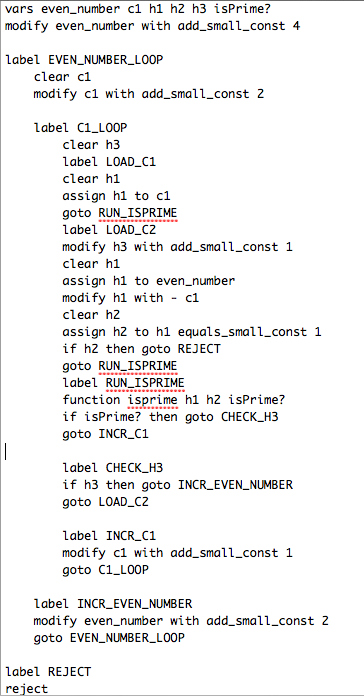
\includegraphics[scale=0.75]{figs/goldbach.png} 
\caption{This is the TMD code for a parsimonious program that will loop if Goldbach's conjecture is true, and reject if it is false. It is provided as an example of a TMD main file. See Figure~\ref{fig:isprime} for the code of the \texttt{isprime} function, which is called by the main body of the program.\label{fig:goldbach}} 
\end{center} 
\end{figure}

\subsection{Function Files}

Function files contain the description of a function. They cannot be run alone; instead, they are called from within a main file or another function file. \\
  
New variables may not be declared from within a function file; instead, any variables needed to perform the computation in the function file are passed in from the file that calls it. Any variables passed into a function file may be modified freely, including integers; that means that there is \emph{no} built-in guarantee that inputs to your function will retain their values after the function runs. \\

Function files may not reach the end of the program without accepting, rejecting, or returning. When a function returns, execution continues at the location of the line beneath where the function was called. Functions never return values; instead, they take effect by modifying the inputs to take on the desired value. \\

Although functions can be called by other functions, they cannot be called recursively (that is, they cannot call themselves and they cannot call functions that eventually call them). This is because the compiler effectively inlines every function when compiling a TMD program to a Turing machine description; no description of a function stack is stored on the tape proper, so a recursive function would cause the compiler to enter an infinite loop. \\

\begin{figure} 
\begin{center} 
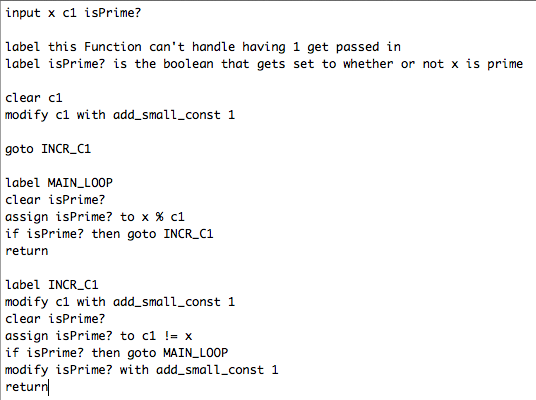
\includegraphics[scale=0.75]{figs/isprime.png} 
\caption{This is the TMD code for a function that will set the value of the input \texttt{isPrime?} to 0 if the input \texttt{x} is not a prime number, and will set the value of \texttt{isPrime?} to a positive integer if \texttt{x} is a prime number. The value of \texttt{x} is not modified by the isprime function, but the value of variable \texttt{c1} may be changed to something arbitrary and the value of \texttt{isPrime?} will be changed to depend on the primality of \texttt{x}. The function's result will depend exclusively on the initial value of \texttt{x}. \label{fig:isprime}} 
\end{center} 
\end{figure}

\subsection{Data Types}

TMD has three possible data types: \texttt{int}, \texttt{list}, and \texttt{list2}. An \texttt{int} is a non-negative integer. A \texttt{list} is a list (possibly empty) of \texttt{int}s. A \texttt{list2} is a list (possibly empty) of \texttt{list}s. TMD is not strongly typed; a variable can at various points belong to various different data types. In fact, it can even belong to multiple data types at once. The \texttt{int} value of \texttt{0}, the \texttt{list} value of \texttt{[]}, and the \texttt{list2} value of \texttt{[]} are all represented the same way on the Turing machine's tape. In accordance with this paradigm, even in the TMD interpreter, if the programmer chose to add \texttt{3} to a variable whose current value was \texttt{0}, it would yield the value \texttt{3}, but if the programmer chose instead to \emph{append} \texttt{3} to a variable whose current value was \texttt{0}, it would yield the value \texttt{[3]}. This is the only situation in which a variable can belong to several different data types simultaneously.

\subsection{Assign Statements}

Assign statements can take any of the following four forms: \\ \\
\texttt{assign x1 to x2} [operation] \texttt{x3} \\ 
\texttt{assign x1 to x2} [operation] \texttt{c} \\
\texttt{assign x1 to x2} [operation] \\
\texttt{assign x1 to x2} \\

Assign statements result in the value of \texttt{x1} being set to the result of the operation [operation] being applied to \texttt{x2} and \texttt{x3} in the first case, to \texttt{x2} and \texttt{c} in the second case, and to \texttt{x2} alone in the third case. In the fourth case, the value of \texttt{x1} is set to the value of \texttt{x2}, as long as \texttt{x2} is an \texttt{int}. Unlike in most programming languages, the value of \texttt{x1} must be 0 before an assign statement can be applied to it. \\

In the explanations that follow, the value of \texttt{x1} is $x_1$, the value of \texttt{x2} is $x_2$, the value of \texttt{x3} is $x_3$, and the value of \texttt{c} is $c$. As before, \texttt{x1}, \texttt{x2}, and \texttt{x3} denote variables, and \texttt{c} denotes a numerical constant. Note that the allowed operations in assign statements are \emph{not} the same as the allowed operations in modify statements. This is because some operations are more parsimonious as an assignment, and other operations are more parsimonious as a modification.

\subsubsection{Multiplication}

\texttt{assign x1 to x2 * x3} \\
implements the operation $x_1 \leftarrow x_2 x_3$. \\ \\
$x_2$ and $x_3$ are required to be \texttt{int}s. \\
After this operation, $x_1$ is an \texttt{int}.

\subsubsection{Division} 

\texttt{assign x1 to x2 / x3} \\
implements the operation $x_1 \leftarrow \left \lfloor{\frac{x_2}{x_3}}\right \rfloor$. \\ \\
$x_2$ and $x_3$ are required to be \texttt{int}s. \\
After this operation, $x_1$ is an \texttt{int}.

\subsubsection{Modulus} 

\texttt{assign x1 to x2 \% x3} \\
implements the operation $x_1 \leftarrow x_2\mod x_3$. \\ \\
$x_2$ and $x_3$ are required to be \texttt{int}s. \\
After this operation, $x_1$ is an \texttt{int}.

\subsubsection{Integer Equality Testing}

\texttt{assign x1 to x2 = x3} \\
implements $x_1 \leftarrow 1$ if and only if $x_2 = x_3$. \\ \\
$x_2$ and $x_3$ are required to be \texttt{int}s. \\
After this operation, $x_1$ is an \texttt{int}.

\subsubsection{Integer Inequality Testing}

\texttt{assign x1 to x2 != x3} \\
implements $x_1 \leftarrow 1$ if and only if $x_2 \not= x_3$. \\ \\
$x_2$ and $x_3$ are required to be \texttt{int}s. \\
After this operation, $x_1$ is an \texttt{int}.

\subsubsection{Constant Equality Testing}

\texttt{assign x1 to x2 equals\_small\_const c} \\
implements $x_1 \leftarrow 1$ if and only if $x_2 = c$. \\ \\
$x_2$ is required to be an \texttt{int}.
After this operation, $x_1$ is an \texttt{int}.

\subsubsection{Comparison (Greater Than)}

\texttt{assign x1 to x2 > x3} \\
implements $x_1 \leftarrow 1$ if and only if $x_2 > x_3$. \\ \\
$x_2$ and $x_3$ are required to be \texttt{int}s. \\
After this operation, $x_1$ is an \texttt{int}.

\subsubsection{Comparison (Less Than)}

\texttt{assign x1 to x2 < x3} \\
implements $x_1 \leftarrow 1$ if and only if $x_2 < x_3$. \\ \\
$x_2$ and $x_3$ are required to be \texttt{int}s. \\
After this operation, $x_1$ is an \texttt{int}.

\subsubsection{List Equality Testing}

\texttt{assign x1 to x2 list\_equals x3} \\
implements $x_1 \leftarrow 1$ if and only if $|x_2| = |x_3|$ and for all integers $0 \le i < |x_2|$, the $i^{\textrm{th}}$ element of $x_2$ equals the $i^{\textrm{th}}$ element of $x_3$. \\ \\
$x_2$ and $x_3$ are required to be \texttt{list}s or \texttt{list2}s. \\
After this operation, $x_1$ is an \texttt{int}. 

\subsubsection{List Index}

\texttt{assign x1 to x2 index x3} \\
implements $x_1 \leftarrow v$, where $v$ is the $x_3^{\textrm{th}}$ value in $x_2$ (0-indexed). \\ \\
$x_2$ is required to be a \texttt{list}, and $x_3$ is required to be an \texttt{int}. \\
After this operation, $x_1$ is an \texttt{int}.

\subsubsection{List2 Index}

\texttt{assign x1 to x2 index2 x3} \\
implements $x_1 \leftarrow v$, where $v$ is the $x_3^{\textrm{th}}$ value in $x_2$ (0-indexed). \\ \\
$x_2$ is required to be a \texttt{list2}, and $x_3$ is required to be an \texttt{int}. \\
After this operation, $x_1$ is a \texttt{list}.

\subsubsection{List Length}

\texttt{assign x1 to x2 length} \\
implements $x_1 \leftarrow |x_2|$. \\ \\ 
$x_2$ is required to be a \texttt{list}. \\
After this operation, $x_1$ is an \texttt{int}.

\subsubsection{List2 Length} 

\texttt{assign x1 to x2 length2} \\
implements $x_1 \leftarrow |x_2|$. \\ \\  
$x_2$ is required to be a \texttt{list2}. \\
After this operation, $x_1$ is an \texttt{int}.

\subsubsection{List Assignment}

\texttt{assign x1 to x2 list} \\
implements $x_1 \leftarrow x_2$. \\ \\  
$x_2$ is required to be a \texttt{list} or \texttt{list2}. \\
After this operation, $x_1$ is a \texttt{list} or a \texttt{list2}.

\subsection{Modify Statements}

Modify statements can take either of the following two forms: \\ \\
\texttt{modify x1 with} [operation] \texttt{x2} \\ 
\texttt{modify x1 with} [operation] \texttt{c} \\

Modify statements result in the value of \texttt{x1} being set to the result of the operation [operation] being applied to \texttt{x1} and \texttt{x2} in the first case, and to \texttt{x1} and \texttt{c} in the second case. \\

In the explanations that follow, the value of \texttt{x1} is $x_1$, the value of \texttt{x2} is $x_2$, and the value of \texttt{c} is $c$. As before, \texttt{x1} and \texttt{x2} denote variables, and \texttt{c} denotes a numerical constant. Note that the allowed operations in assign statements are \emph{not} the same as the allowed operations in modify statements. This is because some operations are more parsimonious as an assignment, and other operations are more parsimonious as a modification.

\subsubsection{Addition}

\texttt{modify x1 with + x2} \\
implements the operation $x_1 \leftarrow x_1 + x_2$. \\ \\
$x_1$ and $x_2$ are required to be \texttt{int}s. \\
After this operation, $x_1$ is an \texttt{int}.

\subsubsection{Subtraction}

\texttt{modify x1 with - x2} \\
implements the operation $x_1 \leftarrow x_1 - x_2$. \\ \\
$x_1$ and $x_2$ are required to be \texttt{int}s. \\
After this operation, $x_1$ is an \texttt{int}.

\subsubsection{Constant Addition}

\texttt{modify x1 with add\_small\_const c} \\
implements the operation $x_1 \leftarrow x_1 + c$. \\ \\
$x_1$ is required to be an \texttt{int}. \\
After this operation, $x_1$ is an \texttt{int}.

\subsubsection{Constant Subtraction}

\texttt{modify x1 with sub\_small\_const c} \\
implements the operation $x_1 \leftarrow x_1 - c$. \\ \\
$x_1$ is required to be an \texttt{int}. \\
After this operation, $x_1$ is an \texttt{int}.

\subsubsection{Appending to Lists}

\texttt{modify x1 with append x2} \\
implements the operation $x_1 \leftarrow x_1 || [x_2]$, where $||$ denotes the concatenation operation. \\ \\
$x_1$ is required to be a \texttt{list}, and $x_2$ is required to be an \texttt{int}. \\
After this operation, $x_1$ is a \texttt{list}.

\subsubsection{Appending to List2s}

\texttt{modify x1 with append2 x2} \\
implements the operation $x_1 \leftarrow x_1 || [x_2]$, where $||$ denotes the concatenation operation. \\ \\
$x_1$ is required to be a \texttt{list2}, and $x_2$ is required to be a \texttt{list}. \\
After this operation, $x_1$ is a \texttt{list2}.

\subsubsection{Appending Constants}

\texttt{modify x1 with append\_small\_const c} \\
implements the operation $x_1 \leftarrow x_1 || [c]$, where $||$ denotes the concatenation operation. \\ \\
$x_1$ is required to be a \texttt{list}. \\
After this operation, $x_1$ is a \texttt{list}.

\subsubsection{List Concatenation}

\texttt{modify x1 with concat x2} \\
implements the operation $x_1 \leftarrow x_1 || x_2$, where $||$ denotes the concatenation operation. \\ \\
$x_1$ and $x_2$ are required to be \texttt{list}s. \\
After this operation, $x_1$ is a \texttt{list}.

\subsubsection{List2 Concatenation}

\texttt{modify x1 with concat2 x2} \\
implements the operation $x_1 \leftarrow x_1 || x_2$, where $||$ denotes the concatenation operation. \\ \\
$x_1$ and $x_2$ are required to be \texttt{list2}s. \\
After this operation, $x_1$ is a \texttt{list2}.

\subsection{Clear Statements}

Clear statements have the following form: \\ \\
\texttt{clear x} \\ \\ 
Clear statements implement the operation $x \leftarrow 0$. \\ \\
Clear statements are often used directly before an assignment to \texttt{x}, because assignment to \texttt{x} requires that $x = 0$. A clear statement can also be used to change the type of \texttt{x}, because \texttt{0} and \texttt{[]} are represented the same way on the Turing machine tape and are treated identically in TMD. Naturally, a clear statement can also be used if the programmer wants to set the value of \texttt{x} to 0. \\

\subsection{Label Statements}

Label statements have the following form: \\ \\ 
\texttt{label L} \\ \\
Label statements do nothing on their own. Instead, label statements \emph{mark} their line of code with their label. For instance, the label statement given above would mark its line of code with the label \texttt{L}. If at some later point, a \texttt{goto} statement is used on the label \texttt{L}, execution will \emph{jump} to whatever line of code contains ``\texttt{label L}.'' In other words, execution will continue at whichever line of code contains ``\texttt{label L}.'' \\ \\
Because label statements have no direct effect, they can also be used for comments. If multiple words follow the \texttt{label} word, all but the first is ignored (and the first becomes the label $L$). \\ \\
Programs cannot contain multiple declarations of the same label.

\subsection{Goto Statements}

Goto statements have the following form: \\ \\
\texttt{goto L} \\ \\ 
When a statement of this form is executed, code execution jumps to whichever line of code contains ``\texttt{label L}.''

\subsection{If-Goto Statements}

If-goto statements have the following form: \\ \\
\texttt{if x goto L} \\ \\ 
When a statement of this form is executed, code execution jumps to whichever line of code contains ``\texttt{label L}'' if \texttt{x} is an \texttt{int} with $x > 0$. If $x = 0$, or if \texttt{x} is a \texttt{list} or a \texttt{list2}, code execution continues to the next line like normal. \\

\subsection{Function Statements}

Function statements have the following form: \\ \\
\texttt{function f x1 x2 x3} \dots \\ \\ 
When a statement of this form is executed, code execution jumps to the top of the function file \texttt{f.tmd}. \texttt{f.tmd} must be in the same directory as whichever file called \texttt{f}. In addition, a mapping is created from the functions' variables to the variables in front of the function call. For example, calling \texttt{function f x1 x2 x3} when \texttt{f.tfn} contains at the top the line \texttt{input x4 x5 x6} will create a mapping from \texttt{x4} to \texttt{x1}, from \texttt{x5} to \texttt{x2}, and from \texttt{x6} to \texttt{x3}. In other words, any operation on \texttt{x4} in \texttt{f.tfn} will in fact be acting on \texttt{x1} from the file that made the function call. This mapping remains in effect until the function returns. \\

Functions cannot be called recursively. In other words, they cannot call themselves, or other functions that eventually call them. Formally, if each function was a node in a graph, and a directed edge was drawn from function \texttt{f1} to function \texttt{f2} if function \texttt{f1} called \texttt{f2}, then that graph cannot contain cycles.

\subsection{Print Statements}

Print statements have the following form: \\ \\ 
\texttt{print x} \\ \\ 
When a statement of this form is executed by the interpreter, ``\texttt{x:}''$|| x$ is printed to the standard output, where $x$ is a string representation of the value of \texttt{x} and $||$ is the string concatenation operation. Statements of this form are ignored by the compiler. Print statements are intended primarily to help debug a program that will later be compiled; the user need not worry about statements like these reducing the parsimony of the resulting compiled Turing machine, because the compiler ignores them during compilation.

\subsection{Halting Statements}

Halting statements have one of the following two forms: \\ \\
\texttt{accept} \\
\texttt{reject} \\ \\

Instructions like these instruct the Turing machine to halt and enter an accepting or a rejecting state, depending on which of these two commands was used. 

\subsection{Variable Declaration Statements}

Variable declaration statements have one of the following two forms: \\ \\
\texttt{var x1} \\
\texttt{vars x1 x2 x3} \dots \\

Variable declaration statements can only be used in main files. In function files, if more variables are required, more variables need to be passed in as arguments to the function. \\

Regardless of their location in the program, variable declaration statements act at the initialization of the program only, and are otherwise ignored. At the initialization of the program, each variable declaration statement acts to initialize each declared variable with a value of 0. In the compiled program, the number of variables declared indicates to the compiler how many tapes to initialize. \\

Depending on the programmer's preference, variables can be declared one at a time with a sequence of \texttt{var} statements, or all at once with a \texttt{vars} statement (or with a mix of the two). Behavior is identical in each of these cases.

\subsection{Function Input Statements}

Function input statements have the following form: \\ \\
\texttt{input x1 x2 x3} \dots \\

An function input statement defines the variables used in a function. In concert with the function call, it also defines a mapping from the names of the variables defined in the input statement to the variable names used in the function call. For example, calling \texttt{function f x1 x2 x3} when \texttt{f.tfn} contains at the top the line \texttt{input x4 x5 x6} will create a mapping from \texttt{x4} to \texttt{x1}, from \texttt{x5} to \texttt{x2}, and from \texttt{x6} to \texttt{x3}. In other words, any operation on \texttt{x4} in \texttt{f.tfn} will in fact be acting on \texttt{x1} from the file that made the function call. This mapping remains in effect until the function returns. \\

Function input statements must appear exactly once in every function file, as the first line of the program. Function input statements may not appear in main files.

\subsection{Return Statements}

Return statements have the following form: \\ \\
\texttt{return} \\

A return statement instructs code execution to exit the function it is currently in and to return to the line below where the function was originally called. Return statements may not appear in main files.

\section{Compilation from TMD to a Multi-Tape Machine \label{sec:turdtotm}}

This section is devoted to describing the algorithm used to compile a TMD program into a multi-tape, 3-symbol Turing machine.

\subsection{Turing Machine Format}

The following is an example of the file format of the multi-tape, 3-symbol Turing machine output by the compiler. \\

Let us suppose that the Turing machine has three states and two tapes. The three symbols in the Turing machine's alphabet are "\texttt{\_}," "\texttt{1}," and "\texttt{E}." The first state's name is "\texttt{StateOne}," the second state's name is "\texttt{StateTwo}," and the third state's name is "\texttt{StateThree}." The first tape's name is "\texttt{TapeA}," and the second tape's name is "\texttt{TapeB}." \\

\texttt{StateOne} is associated with \texttt{TapeA}. \texttt{StateTwo} is associated with \texttt{TapeB}. \texttt{StateThree} is associated with \texttt{TapeA}. \\

Each line defining the Turing machine's behavior in a given state is written as follows: \\

\texttt{[symbol read] -> [next state]; [direction]; [symbol written]} \\

In the actual Turing machine text file, [next state] is replaced by the state that the Turing machine would enter if it read the symbol [symbol read], [direction] is one of \{\texttt{R, L, -}\} and indicates the direction the head would move in, and [symbol written] is one of \{\texttt{\_, 1, E}\} and indicates the symbol that is written on the tape. Note that in the higher-level, multi-tape 3-symbol Turing machine, as indicated by the \texttt{-} symbol, the head can remain in place, (unlike the lowest-level Turing machine around which the Busy Beaver function is defined, where it cannot). 

Figure~\ref{fig:tmexample} shows the example of this Turing machine file. Figure~\ref{fig:behavior} gives a step-by-step depiction of the behavior of this Turing machine for five steps. \\

\begin{figure} 
\begin{center} 
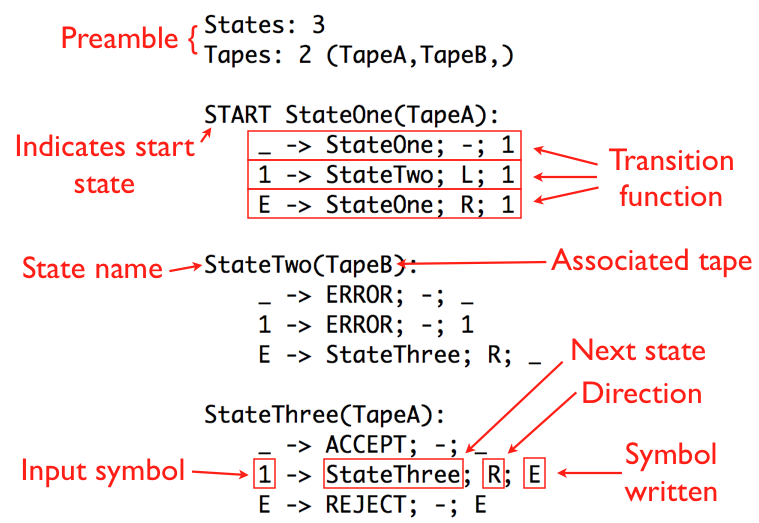
\includegraphics[scale=0.4]{figs/annotatedtm.png} 
\caption{This is an example of a multi-tape Turing machine file. The notes in red are explanations of the meanings of the various parts of the Turing machine file. \label{fig:example}} 
\end{center} 
\end{figure}

\begin{figure} 
\begin{center} 
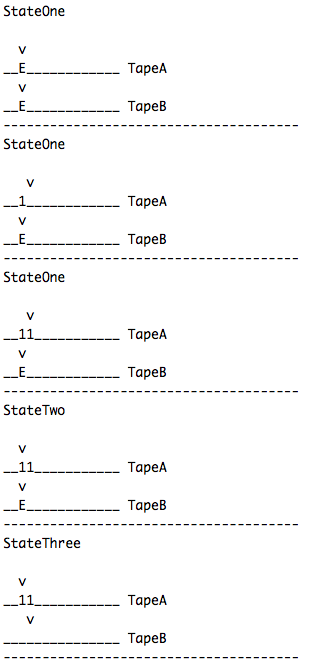
\includegraphics[scale=0.8]{figs/behavior.png} 
\caption{This figure shows the machine shown in Figure~\ref{fig:tmexample} running for five steps. Note that in the multi-tape machine, at initialization, every tape begins with a single \texttt{E} symbol and an infinite number of \texttt{\_} symbols. As will be explained later, this corresponds to every variable having its value be initialized to 0. Naturally, in the lowest-level machine, the tape will be initialized containing only the empty symbol, as required of a standard Turing machine. \label{fig:example}} 
\end{center} 
\end{figure}

In the presented Turing machine, the special halting states \texttt{ACCEPT} and \texttt{REJECT} are used. However, there is an additional halting state that was not previously mentioned: the \texttt{ERROR} state. The \texttt{ERROR} state is not, strictly speaking, necessary to the Turing machines created by my compiler; it is, however, useful for debugging. The core idea of the \texttt{ERROR} state is that the Turing machine should \emph{never enter} it. Situations which should be impossible point to the \texttt{ERROR} state, although in principle they could point to any state while preserving the same functionality. In addition to helping catch bugs in the compiler (because no compiled TMD program that does not throw an error when interpreted should even enter an \texttt{ERROR} state), the \texttt{ERROR} state helps keep lower-level transformation steps parsimonious, as will be described in Sections~\ref{sec:mttost} and~\ref{sec:mstots} Examples where the use of the \texttt{ERROR} states will be mentioned in Section~\ref{sec:compilation}. \\

\subsection{Variable Encoding}

Most of the substance of the general algorithm for compiling a TMD program to a description of a multi-tape Turing machine happens in the encoding of the values of variables. As described earlier, each variable is given its own tape. \\

Because the empty tape symbol is \texttt{\_}, there will at all times be an infinite number of \texttt{\_} symbols on the tape. Therefore, all of the interesting information on the tape must come before the last appearing non-\texttt{\_} symbol. In every encoding of a value on the tape, I guarantee that the last appearing non-\texttt{\_} symbol is the \texttt{E} symbol. I also guarantee that there are no \texttt{\_} symbols that appear in between two non-\texttt{\_} symbols. In other words, the tape is guaranteed to have the following form: $(\texttt{\_})^\infty(\texttt{1}|\texttt{E})^*\texttt{E}(\texttt{\_})^\infty$. These two guarantees will be important in the transformation of the multi-tape machine to a single-tape machine (later, the \texttt{\_} symbol will serve as a separator symbol between different tapes). For the time being, however, these two guarantees serve mainly to constrain the form of the encoding. \\

Integer values are encoded in unary. Specifically, a value of \texttt{0} is encoded with \dots\texttt{\_\_E\_\_}\dots, a value of \texttt{1} is encoded with \dots\texttt{\_\_1E\_\_}\dots, a value of \texttt{2} is encoded with \dots\texttt{\_\_11E\_\_}\dots, and in general a value of $n$ is encoded with $(\texttt{\_})^\infty(\texttt{1})^n\texttt{E}(\texttt{\_})^\infty$. \\

List values are encoded as a sequence of numbers written in unary and broken by \texttt{E} symbols. Specifically, a value of \texttt{[]} is encoded with \dots\texttt{\_\_E\_\_}\dots (note the overlap with the encoding of \texttt{0}), a value of \texttt{[0]} is encoded with \dots\texttt{\_\_E\_\_}\dots, a value of \texttt{[2]} is encoded with \dots\texttt{\_\_E11E\_\_}\dots, and a value of \texttt{[3, 0, 2]} is encoded with \dots\texttt{\_\_E111EE11E\_\_}\dots. In general, a value of $[n_1, n_2, n_3, \dots n_k]$ is encoded with $(\texttt{\_})^\infty\texttt{E}(\texttt{1})^{n_1}\texttt{E}(\texttt{1})^{n_2}\texttt{E}(\texttt{1})^{n_3}\texttt{E}\dots(\texttt{1})^{n_k}\texttt{E}(\texttt{\_})^\infty$. \\

List2 values (lists of lists) are more challenging to encode than lists, because there is not an additional symbol which can be used to break apart the values for lists. The most natural first try is to use \texttt{E} to break between values within a list, and \texttt{EE} to break between different lists. This, however, lends itself to ambiguity, because the \texttt{EE} pattern appears naturally in simple lists that contain \texttt{0}. As an example, using that encoding scheme would result in the same representation for the \texttt{list2} value \texttt{[[3], [2]]} and the \texttt{list2} value \texttt{[[3, 0, 2]]}. \\

In order to fix this issue, the on-tape encoding of \texttt{list2} values increments every stored \texttt{int} value by 1, so that the \texttt{EE} pattern appears only when there is a break between stored \texttt{list}s, and not when a \texttt{list} contains a \texttt{0}. To give a few examples, a value of \texttt{[]} is encoded with \dots\texttt{\_\_E\_\_}\dots, a value of \texttt{[[3, 0], [1, 2]]} is encoded with \dots\texttt{\_\_E1111E1EE11E111EE\_\_}\dots, a value of \texttt{[[]]} is encoded with \dots\texttt{\_\_EE\_\_}\dots, and a value of \texttt{[[2, 4], [], [0]]} is encoded with \dots\texttt{\_\_E111E11111EEE1EE\_\_}\dots. In general, a value of $[[n^1_1, n^1_2, \dots, n^1_{k_1}], [n^2_1, n^2_2, \dots, n^2_{k_2}], \dots, [n^l_1, n^l_2, \dots, n^l_{k_l}]]$ is encoded with: $$(\texttt{\_})^\infty\texttt{E}(\texttt{1})^{n^1_1 + 1}\texttt{E}(\texttt{1})^{n^1_2 + 1}\texttt{E}\dots(\texttt{1})^{n^1_{k_1} + 1}\texttt{EE}(\texttt{1})^{n^2_1 + 1}\texttt{E}(\texttt{1})^{n^2_2 + 1}\texttt{E}\dots(\texttt{1})^{n^2_{k_2} + 1}\texttt{EE}\dots(\texttt{1})^{n^l_1 + 1}\texttt{E}(\texttt{1})^{n^l_2 + 1}\texttt{E}\dots(\texttt{1})^{n^l_{k_l} + 1}\texttt{EE}(\texttt{\_})^\infty$$

\subsection{Compilation \label{compilation}}

Fortunately, compilation itself is a relatively straightforward matter. Lines of code correspond neatly to a single state or a group of states. In between two lines of code, the heads of all involved tapes are required to return to the position of the leftmost non-\texttt{\_} symbol, to retain consistency between situations in which a given line of code may be used. \\

To give an example, the line of code: \\

\texttt{if x goto L}

would correspond to a single state. That state would read the symbol underneath the head associated with \texttt{x}, and if that symbol was a \texttt{1}, the next state would be the first non-empty group of states reached after the line of code containing ``\texttt{label L}.'' If that state was an \texttt{E}, the next state would instead be the first non-empty group of states reached after the line of code below this one.\\

Many lines of code correspond to empty groups of states. For example, \texttt{label} statements, \texttt{goto} statements, variable declaration statements, input statements, and function calls all have empty groups of states associated with them. Such lines of code have no effect on compilation, other than to draw a pointer from the exit states of one group of states to the entrance state of another group of states. \\

The different possible groups of states associated with each possible line of code are too numerous for all of them to be described in detail in this paper. However, to give an example of what a more sophisticated group of states might look like, I present in Figure~\ref{fig:divfsm} the state machine associated with the line of code: \\ \\
\texttt{assign x to y / z} \\

In addition, in Figure~\ref{visualturdtotm}, I present a visual description of compilation from TMD code to a multi-tape Turing machine. \\

% TODO make those figures

\section{Transforming a Multi-Tape Machine to a Single-Tape Machine \label{sec:mttost}}

The output of the compilation process presented in Section~\ref{sec:turdtotm} is a description of a multi-tape Turing machine. Each state in the description has associated with it a tape, and in that state, only that tape is read and modified. The final output of the compilation process is ideally a single-tape machine, to be in line with the standard definition of the Busy Beaver function. Therefore, I present an algorithm for parsimoniously transforming a single-tape Turing machine into a multi-tape Turing machine. \\

It is well-known that a multi-tape Turing machine is ``equivalent'' to a single-tape Turing machine, in the sense that one can simulate the other assuming that an arbitrary overhead in terms of the number of states is allowable. This part of the thesis puts demonstrates the existence of this reduction by giving an explicit algorithm for simulating a multi-tape Turing machine using a single-tape Turing machine. At the same time, this algorithm \emph{minimizes} the overhead in the number of states, unlike many reductions of multi-tape Turing machines to single-tape Turing machines presented in textbooks on complexity theory. Such reductions are often simpler than the one presented in this section, but are unconcerned with the overhead in the number of states and therefore result in a much larger Turing machine. \\

In the descriptions that follow, to avoid confusion between the higher-level tapes of the multi-tape Turing machine and the lower-level tape of the single-tape Turing machine, the higher-level tapes are referred to as \emph{mini-tapes} and the single lower-level-tape is referred to as the \emph{meta-tape}. \\

The transformation described below results in an overhead of about a factor of 10 to 20 in the number of states used in the machine (the exact overhead depends in small part on the number of tapes in the multi-tape machine). 

\subsection{Alphabet}

The single-tape machine's alphabet consists of the three symbols from the multi-tape machine, \texttt{\_}, \texttt{1}, and \texttt{E}, and a new fourth symbol, \texttt{H}. \texttt{H} was introduced in order to be used as a stand-in for the head locations in each of the mini-tape values.

\subsection{Layout}

The transformation from a multi-tape Turing machine to a single-tape Turing machine must necessarily, from an information-theoretic standpoint, store all of the information on each of the many tapes of the multi-tape machine on the single tape. It also must store an identifier of which tape is which. \\

This directly implies what the approximate layout of the single-tape Turing machine must look like. Figure~\ref{fig:stmstmlayout} shows the high-level layout of the Turing machine's tape, with just beneath it a lower-level representation that will be explained in more detail in the following paragraphs. \\

As shown in Figure~\ref{fig:stmstmlayout}, the single tape is occupied by alternating identifiers and values. These identifiers and values are each separated by instances of the \texttt{\_} symbol (which also happens to be the empty symbol). Because the \texttt{\_} symbol is used as a separator and as an indicator that an identifier or a value has been read, the \texttt{\_} is not used inside the identifiers or the values proper. Therefore, identifiers and values draw only from the set of symbols \{\texttt{1}, \texttt{H}, \texttt{E}\}.

The last non-\texttt{\_} on the meta-tape is a \texttt{1}. The only time the \texttt{1\_} pattern appears on the tape signals that the last information on the tape has been read. This will be useful later when attempting to scan the entire tape for a specific value.

\subsection{Identifier Format}

Identifiers are sequences of symbols drawn from \{\texttt{1}, \texttt{H}, \texttt{E}\} that indicate which mini-tape the value to the right of the identifier corresponds to. In other words, the compiler assigns to each mini-tape in the multi-tape Turing machine a unique sequence of \texttt{1}'s, \texttt{H}'s, and \texttt{E}'s. On the meta-tape, to the right of the sequence corresponding to a given mini-tape is that mini-tape's value. \\

On the meta-tape, the \texttt{H\_} pattern indicates the end of an identifier. Therefore, the last non-\texttt{\_} symbol in a valid identifier \emph{must} be \texttt{H}. However, the symbols preceding \texttt{H} in the identifier may be any of \texttt{H}, \texttt{E}, and \texttt{1}, and there may be any number of them. This means that in order to give each variable a unique identifier while making the lengths of identifiers as short as possible and while making the last symbol in each identifier an \texttt{H}, mini-tape identifiers should conform to the following pattern: \\ \\
Mini-tape 1: \texttt{H} \\
Mini-tape 2: \texttt{1H} \\
Mini-tape 3: \texttt{EH} \\
Mini-tape 4: \texttt{HH} \\
Mini-tape 5: \texttt{11H} \\
Mini-tape 6: \texttt{1EH} \\
Mini-tape 7: \texttt{1HH} \\
Mini-tape 8: \texttt{E1H} \\
Mini-tape 9: \texttt{EEH} \\
Mini-tape 10: \texttt{EHH} \\
\dots \\

Having access to three different symbols makes representing mini-tape identifiers as ternary numbers natural. Because there is also flexibility in the size of the number, however, it is best to use every 0-trit ternary number, followed by every 1-trit ternary number, followed by every 2-trit ternary number, and so on. \\

One natural question is: why is it that identifiers should be as short as possible? After all, values in the Turing machine are represented in unary, which is far from the most concise way to represent a number. What motivates the different treatment of identifiers, which are represented in ternary, and values, which are represented in unary? \\

The answer is that the two types of sequences are treated very differently. Values are manipulated, and can often have one of many different possible values. If one is reading an integer $x$ with a value between 1 and $n$, and one wishes to behave differently for each possible value of $x$, $\Omega(n)$ states are necessary to read in $n$'s value, no matter what number system is used to represent $x$. To see that this is true, it suffices to note that if each of the $n$ possible values of $x$ are to lead to a different outcome, then each must lead to a different state--and because a state can only transition to a constant number (in this case, four) of different other states, there must be $\Omega(n)$ states just to lead to $n$ different outcomes. Almost always, in the manipulations of mini-tape values, it is necessary to behave differently for each possible value of $x$. This means that unary is a natural choice for the representations of mini-tape values, because it is otherwise very convenient and simple to use. \\

In contrast, identifiers are generally scanned to see if they are equal to a specific value. If one is reading an integer $x$ with a value between 1 and $n$, and one is only interested in whether or not $x = k$ for some specific other value $k$, then there are only two distinct outcomes: either $x = k$, or $x \not= k$. This means that if $x$ is represented in base 2 or greater, it will be possible to determine which of $x = k$ or $x \not= k$ is true using only $O(\log k)$ states. This is done simply by ``scanning'' the number. To give a concrete example, suppose that we are only interested in whether or not a given identifier is the specific identifier ``\texttt{E1EH}.'' This requires only four states: the first checks that the first symbol is an \texttt{E}, the second checks that the second symbol is a \texttt{1}, and so on. In contrast, if $x$ had been written in unary, determining whether or not $x = k$ would have required $\Omega(k)$ states, since it would have required checking that the first $k$ symbols were all \texttt{1}'s. \\

\subsection{Value Format}

Values are sequences of symbols drawn from \{\texttt{1}, \texttt{H}, \texttt{E}\}. They are meant to represent faithfully the information contained on each mini-tape. Because information on mini-tapes is entirely composed of \texttt{1} and \texttt{E} symbols (although the \texttt{\_} symbol appears on the mini-tapes, it never appears in between two non-\texttt{\_} symbols), the most natural way to represent the information on the mini-tape on the meta-tape is simply to write the symbols from the mini-tape directly onto the meta-tape. \\

This approach successfully records all of the information on the mini-tape except for one part: the location of the mini-tape's head (which I will refer to from now on as the \emph{mini-head}). Recall that each mini-tape has its own head, and that state transitions are possible between states associated with two different mini-tapes, and that each mini-head's location must be remembered in between transitions. This was abstracted away by the higher-level Turing machine representation before, when we assumed that we could have many different tapes and one head for each of them. Now that we are trying to do everything on a single-tape, however, we have only one head to go around. \\

The solution to this issue is the \texttt{H} symbol. The \texttt{H} symbol is always kept immediately to the left of the symbol over which the tape's mini-head would be. Because each mini-tape has only one head, there can only be one \texttt{H} symbol in a mini-tape value at once, the location of which represents the mini-head's location. The mini-tape value representation on the meta-tape is otherwise symbol-for-symbol identical to the sequence of symbols on the higher-level mini-tape.

\subsection{Value Expansion}

The high-level diagram in Figure~\ref{stmstmlayout} obscures an important detail that complicates this transformation. The issue is that although the diagram appears to allocate a fixed block of the meta-tape to each identifier and each mini-tape value, no fixed number of tape slots can suffice to hold a mini-tape value. Because tape identifiers are static (they are drawn on the tape at initialization and never changed again), tape identifiers can be contained in a fixed number of tape slots. Mini-tape values, however, can get arbitrarily large; this means that they potentially need an arbitrarily large amount of space allocated to them. \\

The solution is to dynamically increase the space allocated to a mini-tape value whenever the mini-tape value increases in size. In other words, whenever a state in the multi-tape Turing machine is instructed to write a non-\texttt{\_} symbol on top of a \texttt{\_} symbol, it enters a group of intermediate states designed to ``push'' every symbol down along the tape, to create one more symbol of room for the mini-tape value. This group of intermediate states remembers the symbol it just read, moves right, writes down the symbol it just read, and repeats. See Figure~\ref{fig:expandfsm} for a diagram of the state machine used to ``push'' every symbol along the tape and make room for the expanding mini-tape value. \\

\subsection{Overview of Transformation}

Now that the high-level ideas have been described in detail, a step-by-step low-level description of the transformmation process can be given. \\

Suppose that the multi-tape Turing machine contains an instruction of the form: \\

\emph{When in State $S_a$ (associated with Tape $T_a$), if symbol $r$ is read, write the symbol $w$ on the tape, move the head in direction $d$, and enter State $S_b$ (associated with Tape $T_b$).} \\

In the single-tape Turing machine, this instruction will take many more states to represent, and will follow one of the series of instructions below, depending on the values of $r$, $w$, $T_a$, and $T_b$. \\

\textbf{If $r = \texttt{\_}$ and $w \not= \texttt{\_}$:}

\begin{enumerate}

\item Read the symbol below the meta-head. If that symbol is $r$, write $w$.
\item If the $d$ is an instruction not to move the mini-head, do nothing. Otherwise, swap the \texttt{H} symbol on the tape with the symbol to its left or right, depending on whether $d$ is ``left'' or ``right.''
\item Go right until the first \texttt{\_} symbol is found. Write a \texttt{\_} symbol onto the tape, and ``push'' every symbol to the right down one space on the meta-tape by remembering the symbol that was just read, moving right, writing the remembered symbol, and repeating. Do this until the \texttt{1\_} pattern is encountered, which signals the end of the information on the meta-tape.
\item Move the meta-head left, scanning for the sequence of symbols that corresponds to the identifier for tape $T_b$.
\item After the identifier has been reached, move the meta-head right until the \texttt{H\_} pattern is encountered, which signals the end of the identifier.
\item Move the meta-head right until the \texttt{H} symbol is encountered, which indicates the head is one symbol to the right. Move the meta-head right once more.

\end{enumerate}

\textbf{If $r \not= \texttt{\_}$ or $w = r$, and also $T_a \not= T_b$:}

\begin{enumerate}

\item Read the symbol below the meta-head. If that symbol is $r$, write $w$.
\item If the $d$ is an instruction not to move the mini-head, do nothing. Otherwise, swap the \texttt{H} symbol on the tape with the symbol to its left or right, depending on whether $d$ is ``left'' or ``right.''
\item Move the meta-head right until the \texttt{1\_} pattern is encountered, which signals the end of the information on the meta-tape.
\item Move the meta-head left, scanning for the sequence of symbols that corresponds to the identifier for tape $T_b$.
\item After the identifier has been reached, move the meta-head right until the \texttt{H\_} pattern is encountered, which signals the end of the identifier.
\item Move the meta-head right until the \texttt{H} symbol is encountered, which indicates the head is one symbol to the right. Move the meta-head right once more.

\end{enumerate}

\textbf{If $r \not= \texttt{\_}$ or $w = r$, and also $T_a = T_b$} (this case is special because the meta-head need not leave the mini-tape representation that it started on):
\begin{enumerate}

\item Read the symbol below the meta-head. If that symbol is $r$, write $w$.
\item If the $d$ is an instruction not to move the mini-head, do nothing. Otherwise, swap the \texttt{H} symbol on the tape with the symbol to its left or right, depending on whether $d$ is ``left'' or ``right.'' After swapping, move the meta-head one symbol to the right of the new \texttt{H} symbol.

\end{enumerate}

\section{Transforming a 4-Symbol Machine to a 2-Symbol Machine \label{sec:mstots}}

The output of the transformation process presented in Section~\ref{sec:mttost} is a description of a 4-symbol Turing machine. While some definitions of the Busy Beaver function allow for a variable-size alphabet, the standard definition requires the alphabet to contain only two symbols. This means that an additional transformation step is necessary to turn the 4-symbol Turing machine into a 2-symbol machine. \\

Like the transformation described in Section~\ref{sec:mttost}, the equivalence of Turing machines with differently-sized finite alphabets is well-known. Unlike the transformation described in Section~\ref{sec:mttost}, common proofs of their equivalence tend to use the same techniques as the one described here. The general idea is to assign to each symbol in the larger alphabet an equivalent sequence of symbols in the smaller alphabet. \\

The transformation described below results in an overhead of about a factor of 20 in the number of states used in the machine.

\subsection{Alphabet}

The alphabet of the 2-symbol machine contains two symbols, which I decided to call \texttt{a} and \texttt{b}, because they don't map neatly to \texttt{0} and \texttt{1}, and because the \texttt{1} symbol was already used in the 4-symbol alphabet. \\

The mapping from \{\texttt{\_}, \texttt{1}, \texttt{H}, \texttt{E}\} to sequences of symbols from \{\texttt{a}, \texttt{b}\} is as follows: \\ \\
\texttt{\_} $\leftrightarrow$ \texttt{aa} \\
\texttt{1} $\leftrightarrow$ \texttt{ab} \\
\texttt{H} $\leftrightarrow$ \texttt{ba} \\
\texttt{E} $\leftrightarrow$ \texttt{bb} \\

\texttt{a} is the empty symbol.

\subsection{Overview of Transformation}

The following is a step-by-step low-level description of the transformation process. \\

Suppose that the 4-symbol Turing machine contains an instruction of the form: \\

\emph{When in State $S_a$, if symbol $r$ is read, write the symbol $w$ on the tape, move the head in direction $d$, and enter State $S_b$.} \\

In the 2-symbol Turing machine, this instruction will take many more states to represent, and will follow one of the series of instructions below, depending on the values of $r$ and $w$. \\

\textbf{If $r = w$:}

\begin{enumerate}

\item Read the symbol below the head. Remember the symbol that was read, move right, and read the new symbol that is under the head. 
\item If the two symbols read in map to $r$, move three spaces left, one space left, or one space right, depending on whether $d$ is an instruction to move left, stay in place, or move right, respectively.

\end{enumerate}

\textbf{If $r \not= w$:}

\begin{enumerate}

\item Read the symbol below the head. Remember the symbol that was read, move right, and read the new symbol that is under the head.
\item Let $w_1$ be the first symbol in the sequence of symbols that that map to $w$, and let $w_2$ be the second symbol in that same sequence. If the two symbols read in map to $r$, write $w_2$, move left, and write $w_1$.
\item Move two spaces left, move left and then right, or move two spaces right, depending on whether $d$ is an instruction to move left, stay in place, or move right, respectively.

\end{enumerate}

Note that although the higher-level Turing machines with more than 2-symbol alphabets allow the head to stay in place, the bottom-most representation does not, which is important: in the standard definition of the Busy Beaver function, the head must move left or right at each step and cannot stay in place.

% TODO elaborate on possible optimizations to the mstots compiler?

\section{Miscellaneous Optimizations}

\subsection{Pruning}

The output of the compiler as presented sometimes contains states where both possible transitions out of the state lead to the error state. In this case, the states in question are clearly themselves equivalent to the error state, and can be replaced with the error state, thereby reducing the number of states in the final Turing machine. Running this simple optimization on the Turing machine reduces the state usage of the final Turing machine by about 5\%.

% TODO: make the code use ternary and H_

% TODO conclusion?

\end{document}

